\chapter{Weiche repulsive Teilchen in 2D in periodischer Simulationsbox}
Da nun die grundlegenden Eigenschaften der Simulation getestet sind, wird die Simulation dahingehend erweitert, dass sie als Modell f�r eine Lennard-Jones-Fl�ssigkeit dienen kann.

\section{Zellunterteilung}
Da die im vorherigen Kapitel bestimmte Laufzeit von $O(N^2)$ f�r Simulationen mit vielen Teilchen ungeeignet ist, wird die vorhandene Simulation im Bezug auf die Laufzeit optimiert. Da der aufw�ndigste Schritt die Berechnung der Kraft auf jedes Teilchen ist - hierzu muss gegen alle andere (N-1)-Teilchen getestet werden -, setzt die Optimierung hier an. Dazu wird das Lennard-Jones-Potenzial angepasst. Da der absto�ende Teil des Potenzials st�rkere Kr�fte erzeugt, wird das Potential auf diesen Teil eingeschr�nkt. Das ver�nderte Potential hat dadurch folgende Form.
\begin{equation}
V(r) = \left\{ 
\begin{array}{lll} 
4\epsilon \left[\left(\frac{\sigma}{r}\right)^{12} - \left(\frac{\sigma}{r}\right)^6 \right] + \epsilon& \quad \text{f�r} & r<r_c \\  
0 & \quad\text{f�r} & r \geq r_c 
\end{array}
\right.
\end{equation}
$r_c$ bezeichnet dabei wie in \fref{chap:LJ} beschrieben, das Minimum des Potentials. Dieses wurde durch die Modifikation nicht ver�ndert. Genauso ist auch die Kraft unver�ndert, bis auf das, dass der anziehende Teil durch die zus�tzliche Bedingung abgeschnitten wurde. Die H�he des Potentials wurde so ver�ndert, dass es stetig gegen 0 ausl�uft.

Da die Teilchen, die nun diesem Potential unterliegen, keine "`Oberfl�chenspannung"' mehr besitzen, das hei�t, sich nicht mehr gegenseitig anziehen, expandiert das System vom Startpunkt aus. Da auch die Teilchen in der Mitte der Substanz in der Realit�t keine Oberfl�chenspannung mehr sp�ren, ist dieses Modell, f�r das Innere der Substanz, durchaus angebracht. Die Teilchen werden dabei aber von ihren Nachbarn nahe ihrer Position gehalten. Da das simulierte System aber endlich ist, expandiert es. Um dies zu beheben, werden die Teilchen in eine Box eingesperrt, in der periodische Randbedingungen herrschen. Das hei�t, die Teilchen, die die Box rechts verlassen, kommen links wieder in die Box herein und sp�ren auch die absto�enden Kr�fte �ber die Boxwand hinweg. Die Dimension der Box wird so gew�hlt, dass sie einer Einheitszelle entspricht.

Da das Potential nun nur noch f�r Abst�nde $<r_c$ Auswirkungen hat, lassen sich die ben�tigten Teilchen-Teilchen-Wechselwirkungen auf Teilchen im Umkreis von $r_c$ um das Teilchen reduzieren. Technisch wird dies dadurch gel�st, dass die Box in kleine Zellen mit der Breite $r_c$ eingeteilt wird, in die die Teilchen nach jedem Schritt einsortiert werden. Bei der Berechnung der Wechselwirkung werden nun nur noch angrenzenden Zellen beachtet. Dies reduziert die Komplexit�t des Programms auf $O(N)$. Um dies zu �berpr�fen, wird wie im vorherigen Kapitel die Komplexit�t ermittelt.
\begin{figure}[h!]
	\centering
		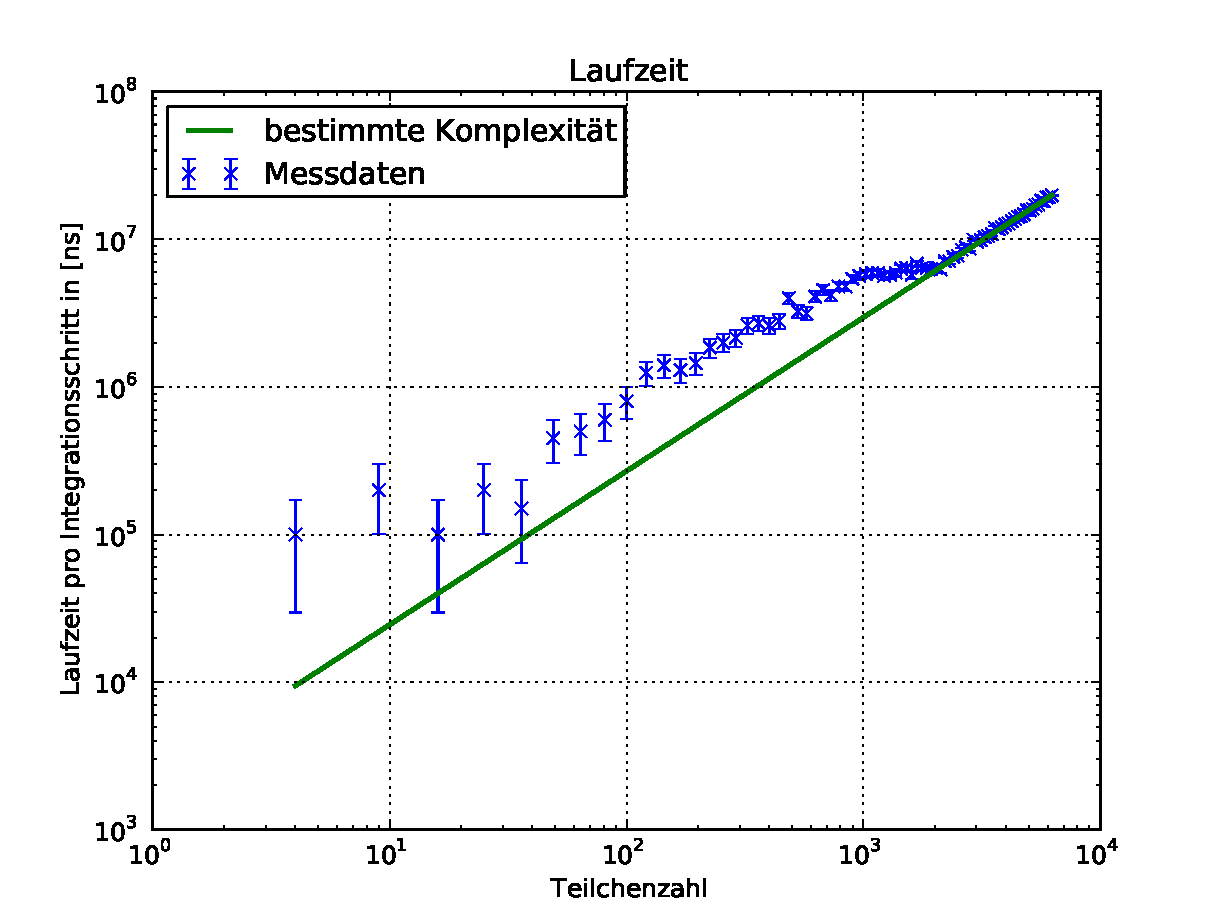
\includegraphics[width=0.70\textwidth]{img/LZCS.pdf}
	\caption{Laufzeit der Simulation mit implementierter Zellunterteilung in Abh�ngigkeit von der Teilchenzahl mit polynomialen Fit. Es zeigt sich eine $N$ Abh�ngigkeit.}
	\label{fig:LZCS}
\end{figure}
Der Geradenfit ergibt dieses Mal \textbf{1.05}, was sehr gut mit unseren �berlegungen �bereinstimmt.

\section{Energieerhaltung}
Um die Energieerhaltung gegen�ber dem Eulerverfahren zu verbessern, wird auf ein anderes Integrationsverfahren umgestiegen. Dieses Verfahren nennt sich Leap-Frog-Verfahren und ist wie folgt definiert:
\begin{align}
x_{t+\Delta t} &= x_t + \dot{x}_{t+0.5\Delta t} \Delta t \\
\dot{x}_{t+\Delta t} &= \dot{x}_t + \ddot{x}_{t+0.5\Delta t} \Delta t 
\end{align}
Der Unterschied zum Eulerverfahren besteht darin, die erste Ableitung nicht an der Stelle $t$ sondern an der Stelle $t+0.5\Delta t$ zu berechnen. Dies hat eine wesentlich bessere Konvergenz der Trajektorien zur Folge. \cite[Kap. 3.5]{rapaport2004} Im Gegensatz zum noch genaueren Runge-Kutta-Verfahren kommt das Leap-Frog-Verfahren aber mit nur einer Auswertung des Kraft aus. Da Runge-Kutta-Verfahren ben�tigt f�r jeden Schritt vier Auswertungen. Da die Auswertung der Kraft der zeitaufw�ndigste Teil der Simulation ist, wird die Ungenauigkeit zu Gunsten der k�rzeren Rechenzeit in Kauf genommen.